% Autor: Kamil Ziemian

% --------------------------------------------------------------------
% Podstawowe ustawienia i pakiety
% --------------------------------------------------------------------
\RequirePackage[l2tabu, orthodox]{nag}  % Wykrywa przestarzałe i niewłaściwe
% sposoby używania LaTeXa. Więcej jest w l2tabu English version.
\documentclass[a4paper,11pt]{article}
% {rozmiar papieru, rozmiar fontu}[klasa dokumentu]
\usepackage[MeX]{polski}  % Polonizacja LaTeXa, bez niej będzie pracował
% w języku angielskim.
\usepackage[utf8]{inputenc} % Włączenie kodowania UTF-8, co daje dostęp
% do polskich znaków.
\usepackage{lmodern}  % Wprowadza fonty Latin Modern.
\usepackage[T1]{fontenc}  % Potrzebne do używania fontów Latin Modern.



% ----------------------------
% Podstawowe pakiety (niezwiązane z ustawieniami języka)
% ----------------------------
\usepackage{microtype}  % Twierdzi, że poprawi rozmiar odstępów w tekście.
\usepackage{graphicx}  % Wprowadza bardzo potrzebne komendy do wstawiania
% grafiki.
% \usepackage{verbatim}  % Poprawia otoczenie VERBATIME.
% \usepackage{textcomp}  % Dodaje takie symbole jak stopnie Celsiusa,
% wprowadzane bezpośrednio w tekście.
\usepackage{vmargin}  % Pozwala na prostą kontrolę rozmiaru marginesów,
% za pomocą komend poniżej. Rozmiar odstępów jest mierzony w calach.
% ----------------------------
% MARGINS
% ----------------------------
\setmarginsrb
{ 0.7in} % left margin
{ 0.6in} % top margin
{ 0.7in} % right margin
{ 0.8in} % bottom margin
{  20pt} % head height
{0.25in} % head sep
{   9pt} % foot height
{ 0.3in} % foot sep



% ------------------------------
% Często przydatne pakiety
% ------------------------------
% \usepackage{csquotes}  % Pozwala w prosty sposób wstawiać cytaty do tekstu.
% \usepackage{xcolor}  % Pozwala używać kolorowych czcionek (zapewne dużo
% więcej, ale ja nie potrafię nic o tym powiedzieć).




% ------------------------------
% Pakiety do tekstów z nauk przyrodniczych
% ------------------------------
\let\lll\undefined  % Amsmath gryzie się z pakietami do języka
% polskiego, bo oba definiują komendę \lll. Aby rozwiązać ten problem
% oddefiniowuję tę komendę, ale może tym samym pozbywam się dużego Ł.
\usepackage[intlimits]{amsmath}  % Podstawowe wsparcie od American
% Mathematical Society (w skrócie AMS)
\usepackage{amsfonts, amssymb, amscd, amsthm}  % Dalsze wsparcie od AMS
% \usepackage{siunitx}  % Do prostszego pisania jednostek fizycznych
\usepackage{upgreek}  % Ładniejsze greckie litery
% Przykładowa składnia: pi = \uppi
% \usepackage{slashed}  % Pozwala w prosty sposób pisać slash Feynmana.
\usepackage{calrsfs}  % Zmienia czcionkę kaligraficzną w \mathcal
% na ładniejszą. Może w innych miejscach robi to samo, ale o tym nic
% nie wiem.



% ------------------
% TikZ
% ------------------
\usepackage{tikz}  % Potężny pakiet PGF/TikZ.
\usetikzlibrary{arrows.meta}
\usetikzlibrary{positioning}
\usetikzlibrary{bending}
\usetikzlibrary{graphs}
\usetikzlibrary{patterns}



% ----------
% Tworzenie otoczeń "Twierdzenie", "Definicja", "Lemat", etc.
% ----------
\newtheorem{twr}{Twierdzenie}  % Komenda wprowadzająca otoczenie
% ,,twr'' do pisania twierdzeń matematycznych
\newtheorem{defin}{Definicja}  % Analogicznie jak powyżej
\newtheorem{wni}{Wniosek}



% ----------------------------
% Pakiety napisane przez użytkownika.
% Mają być w tym samym katalogu to ten plik .tex
% ----------------------------
% \usepackage{analizamatematyczna}  % Pakiet napisany między innymi
% % dla tego pliku.
\usepackage{latexshortcuts}
\usepackage{mathshortcuts}




% --------------------------------------------------------------------
% Dodatkowe ustawienia dla języka polskiego
% --------------------------------------------------------------------
\renewcommand{\thesection}{\arabic{section}.}
% Kropki po numerach rozdziału (polski zwyczaj topograficzny)
\renewcommand{\thesubsection}{\thesection\arabic{subsection}}
% Brak kropki po numerach podrozdziału



% ----------------------------
% Ustawienia różnych parametrów tekstu
% ----------------------------
\renewcommand{\arraystretch}{1.2}  % Ustawienie szerokości odstępów między
% wierszami w tabelach.



% ----------------------------
% Pakiet "hyperref"
% Polecano by umieszczać go na końcu preambuły.
% ----------------------------
\usepackage{hyperref}  % Pozwala tworzyć hiperlinki i zamienia odwołania
% do bibliografii na hiperlinki.





% --------------------------------------------------------------------
% Tytuł, autor, data
\title{Ti\emph{k}Z \& PGF \\
  \href{http://piotrkosoft.net/pub/mirrors/CTAN/graphics/pgf/base/doc/pgfmanual.pdf}{Manual for version 3.1.4.} \\
  Series 01, file 04}

\author{}



% \date{}
% --------------------------------------------------------------------







% ####################################################################
\begin{document}
% ####################################################################



% ######################################
\maketitle % Tytuł całego tekstu
% ######################################



% ######################################
\section{16.3.7 Line Styling}

\vspace{2em}

% ######################################



% ##################
\begin{figure}[ht]
  \centering

  
\begin{tikzpicture}[line width=2mm]
    \draw [arrows = {-Computer Modern Rightarrow[line cap=butt]}]
    (0,0) -- (1,0);
  \end{tikzpicture}

  \caption{Ti\emph{k}Z 1.}
\end{figure}
% ##################





% ##################
\begin{figure}[ht]
  \centering

  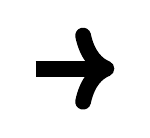
\begin{tikzpicture}[line width=2mm]
    \draw [arrows = {-Computer Modern Rightarrow[line cap=round]}]
    (0,0) -- (1,0);
  \end{tikzpicture}

  \caption{Ti\emph{k}Z 2.}
\end{figure}
% ##################





% ##################
\begin{figure}[ht]
  \centering

  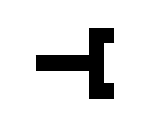
\begin{tikzpicture}[line width=2mm]
    \draw [arrows = {-Bracket[reversed,line cap=butt]}]
    (0,0) -- (1,0);
  \end{tikzpicture}

  \caption{Ti\emph{k}Z 3.}
\end{figure}
% ##################





% ##################
\begin{figure}[ht]
  \centering

  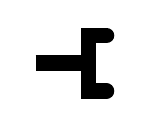
\begin{tikzpicture}[line width=2mm]
    \draw [arrows = {-Bracket[reversed,line cap=round]}]
    (0,0) -- (1,0);
  \end{tikzpicture}

  \caption{Ti\emph{k}Z 4.}
\end{figure}
% ##################





% ##################
\begin{figure}[ht]
  \centering

  
\begin{tikzpicture}[line width=2mm]
    \draw [arrows = {-Computer Modern Rightarrow[line join=miter]}]
    (0,0) -- (1,0);
  \end{tikzpicture}

  \caption{Ti\emph{k}Z 5.}
\end{figure}
% ##################





% ##################
\begin{figure}[ht]
  \centering

  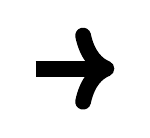
\begin{tikzpicture}[line width=2mm]
    \draw [arrows = {-Computer Modern Rightarrow[line join=round]}]
    (0,0) -- (1,0);
  \end{tikzpicture}

  \caption{Ti\emph{k}Z 6.}
\end{figure}
% ##################





% ##################
\begin{figure}[ht]
  \centering

  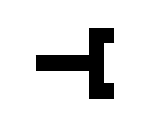
\begin{tikzpicture}[line width=2mm]
    \draw [arrows = {-Bracket[reversed,line join=miter]}]
    (0,0) -- (1,0);
  \end{tikzpicture}

  \caption{Ti\emph{k}Z 7.}
\end{figure}
% ##################





% ##################
\begin{figure}[ht]
  \centering

  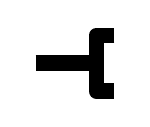
\begin{tikzpicture}[line width=2mm]
    \draw [arrows = {-Bracket[reversed,line join=round]}]
    (0,0) -- (1,0);
  \end{tikzpicture}

  \caption{Ti\emph{k}Z 8.}
\end{figure}
% ##################





% ##################
\begin{figure}[ht]
  \centering

  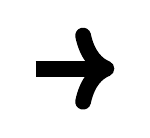
\begin{tikzpicture}[line width=2mm]
    \draw [arrows = {-Computer Modern Rightarrow[round]}]
    (0,0) -- (1,0);
  \end{tikzpicture}

  \caption{Ti\emph{k}Z 9.}
\end{figure}
% ##################





% ##################
\begin{figure}[ht]
  \centering

  
\begin{tikzpicture}[line width=2mm]
    \draw [arrows = {-Bracket[reversed,round]}] (0,0) -- (1,0);
  \end{tikzpicture}

  \caption{Ti\emph{k}Z 10.}
\end{figure}
% ##################





% ##################
\begin{figure}[ht]
  \centering

  
\begin{tikzpicture}[line width=2mm]
    \draw [arrows = {-Computer Modern Rightarrow[sharp]}] (0,0) -- (1,0);
  \end{tikzpicture}

  \caption{Ti\emph{k}Z 11.}
\end{figure}
% ##################





% ##################
\begin{figure}[ht]
  \centering

  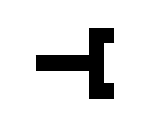
\begin{tikzpicture}[line width=2mm]
    \draw [arrows = {-Bracket[reversed,sharp]}] (0,0) -- (1,0);
  \end{tikzpicture}

  \caption{Ti\emph{k}Z 12.}
\end{figure}
% ##################





% ##################
\begin{figure}[ht]
  \centering

  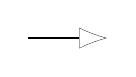
\begin{tikzpicture}
    \draw [arrows = {-Latex[line width=0.1pt, fill=white, length=10pt]}]
    (0,0) -- (1,0);
  \end{tikzpicture}

  \caption{Ti\emph{k}Z 13.}
\end{figure}
% ##################





% ##################
\begin{figure}[ht]
  \centering

  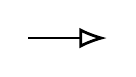
\begin{tikzpicture}
    \draw [arrows = {-Latex[line width=1pt, fill=white, length=10pt]}]
    (0,0) -- (1,0);
  \end{tikzpicture}

  \caption{Ti\emph{k}Z 14.}
\end{figure}
% ##################





% ##################
\begin{figure}[ht]
  \centering

  \def\wall{ \fill [fill=black!50] (1,-0.5) rectangle (2,0.5);
    \pattern [pattern=bricks] (1,-0.5) rectangle (2,0.5);
    \draw [line width=1pt] (1cm+0.5pt,-0.5) -- ++(0,1);
  }

  
\begin{tikzpicture}
    \wall

    % The "line"
    \draw [red,line width=1mm] (-1,0) -- (1,0);
  \end{tikzpicture}

  \caption{Ti\emph{k}Z 15.}
\end{figure}
% ##################





% ##################
\begin{figure}[ht]
  \centering

  \def\wall{ \fill [fill=black!50] (1,-0.5) rectangle (2,0.5);
    \pattern [pattern=bricks] (1,-0.5) rectangle (2,0.5);
    \draw [line width=1pt] (1cm+0.5pt,-0.5) -- ++(0,1);
  }

  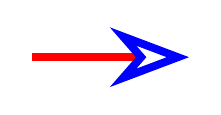
\begin{tikzpicture}
    \wall

    \draw [red,line width=1mm,-{Stealth[length=1cm,open,blue]}]
    (-1,0) -- (1,0);
  \end{tikzpicture}

  \caption{Ti\emph{k}Z 16.}
\end{figure}
% ##################





% ##################
\begin{figure}[ht]
  \centering

  \def\wall{ \fill [fill=black!50] (1,-0.5) rectangle (2,0.5);
    \pattern [pattern=bricks] (1,-0.5) rectangle (2,0.5);
    \draw [line width=1pt] (1cm+0.5pt,-0.5) -- ++(0,1);
  }

  
\begin{tikzpicture}
    \wall

    \draw [red!25,line width=1mm] (-1,0) -- (1,0);

    \draw [red,line width=1mm]
    (-1,-0.5) .. controls (0,-0.5) and (0,0) .. (1,0);
  \end{tikzpicture}

  \caption{Ti\emph{k}Z 17.}
\end{figure}
% ##################





% ##################
\begin{figure}[ht]
  \centering

  \def\wall{ \fill [fill=black!50] (1,-0.5) rectangle (2,0.5);
    \pattern [pattern=bricks] (1,-0.5) rectangle (2,0.5);
    \draw [line width=1pt] (1cm+0.5pt,-0.5) -- ++(0,1);
  }

  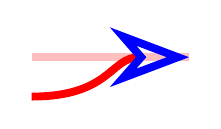
\begin{tikzpicture}
    \wall

    \draw [red!25,line width=1mm] (-1,0) -- (1,0);

    \draw [red,line width=1mm,-{Stealth[length=1cm,open,blue,quick]}]
    (-1,-0.5) .. controls (0,-0.5) and (0,0) .. (1,0);
  \end{tikzpicture}

  \caption{Ti\emph{k}Z 18.}
\end{figure}
% ##################





% ##################
\begin{figure}[ht]
  \centering

  \def\wall{ \fill [fill=black!50] (1,-0.5) rectangle (2,0.5);
    \pattern [pattern=bricks] (1,-0.5) rectangle (2,0.5);
    \draw [line width=1pt] (1cm+0.5pt,-0.5) -- ++(0,1);
  }

  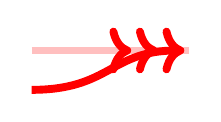
\begin{tikzpicture}
    \wall

    \draw [red!25,line width=1mm] (-1,0) -- (1,0);

    \draw [red,line width=1mm,-{[quick,sep]>>>}]
    (-1,-0.5) .. controls (0,-0.5) and (0,0) .. (1,0);
  \end{tikzpicture}

  \caption{Ti\emph{k}Z 19.}
\end{figure}
% ##################


Strona 200 bending.


% % ##################
% \begin{figure}[ht]
%   \centering

%   \begin{tikzpicture}

%   \end{tikzpicture}

%   \caption{Ti\emph{k}Z .}
% \end{figure}
% % ##################





% % ##################
% \begin{figure}[ht]
%   \centering

%   \begin{tikzpicture}

%   \end{tikzpicture}

%   \caption{Ti\emph{k}Z .}
% \end{figure}
% % ##################





% % ##################
% \begin{figure}[ht]
%   \centering

%   \begin{tikzpicture}

%   \end{tikzpicture}

%   \caption{Ti\emph{k}Z .}
% \end{figure}
% % ##################





% % ##################
% \begin{figure}[ht]
%   \centering

%   \begin{tikzpicture}

%   \end{tikzpicture}

%   \caption{Ti\emph{k}Z .}
% \end{figure}
% % ##################





% % ##################
% \begin{figure}[ht]
%   \centering

%   \begin{tikzpicture}

%   \end{tikzpicture}

%   \caption{Ti\emph{k}Z .}
% \end{figure}
% % ##################





% % ##################
% \begin{figure}[ht]
%   \centering

%   \begin{tikzpicture}



%   \end{tikzpicture}

%   \caption{Ti\emph{k}Z .}
% \end{figure}
% % ##################





% % ##################
% \begin{figure}[ht]
%   \centering

%   \begin{tikzpicture}



%   \end{tikzpicture}

%   \caption{Ti\emph{k}Z .}
% \end{figure}
% % ##################





% % ##################
% \begin{figure}[ht]
%   \centering

%   \begin{tikzpicture}



%   \end{tikzpicture}

%   \caption{Ti\emph{k}Z .}
% \end{figure}
% % ##################





% % ##################
% \begin{figure}[ht]
%   \centering

%   \begin{tikzpicture}

%   \end{tikzpicture}

%   \caption{Ti\emph{k}Z .}
% \end{figure}
% % ##################





% % ##################
% \begin{figure}[ht]
%   \centering

%   \begin{tikzpicture}


%   \end{tikzpicture}

%   \caption{Ti\emph{k}Z .}
% \end{figure}
% % ##################





% % ##################
% \begin{figure}[ht]
%   \centering

%   \begin{tikzpicture}


%   \end{tikzpicture}

%   \caption{Ti\emph{k}Z .}
% \end{figure}
% % ##################





% % ##################
% \begin{figure}[ht]
%   \centering

%   \begin{tikzpicture}




%   \end{tikzpicture}

%   \caption{Ti\emph{k}Z .}
% \end{figure}
% % ##################





% % ##################
% \begin{figure}[ht]
%   \centering

%   \begin{tikzpicture}




%   \end{tikzpicture}

%   \caption{Ti\emph{k}Z .}
% \end{figure}
% % ##################





% % ##################
% \begin{figure}[ht]
%   \centering

%   \begin{tikzpicture}

%   \end{tikzpicture}

%   \caption{Ti\emph{k}Z .}
% \end{figure}
% % ##################





% % ##################
% \begin{figure}[ht]
%   \centering

%   \begin{tikzpicture}





%   \end{tikzpicture}

%   \caption{Ti\emph{k}Z .}
% \end{figure}
% % ##################





% % ##################
% \begin{figure}[ht]
%   \centering

%   \begin{tikzpicture}





%   \end{tikzpicture}

%   \caption{Ti\emph{k}Z .}
% \end{figure}
% % ##################





% % ##################
% \begin{figure}[ht]
%   \centering

%   \begin{tikzpicture}



%   \end{tikzpicture}

%   \caption{Ti\emph{k}Z .}
% \end{figure}
% % ##################





% % ##################
% \begin{figure}[ht]
%   \centering

%   \begin{tikzpicture}





%   \end{tikzpicture}

%   \caption{Ti\emph{k}Z .}
% \end{figure}
% % ##################





% % ##################
% \begin{figure}[ht]
%   \centering

%   \begin{tikzpicture}





%   \end{tikzpicture}

%   \caption{Ti\emph{k}Z .}
% \end{figure}
% % ##################





% % ##################
% \begin{figure}[ht]
%   \centering

%   \begin{tikzpicture}





%   \end{tikzpicture}

%   \caption{Ti\emph{k}Z .}
% \end{figure}
% % ##################





% % ##################
% \begin{figure}[ht]
%   \centering

%   \begin{tikzpicture}





%   \end{tikzpicture}

%   \caption{Ti\emph{k}Z .}
% \end{figure}
% % ##################





% % ##################
% \begin{figure}[ht]
%   \centering

%   \begin{tikzpicture}
%     \draw[arrows = {-Stealth[]}] (0,1) -- (1,1);

%     \draw[arrows = {-Stealth[scale width=1.5]}] (0,0.5) -- (1,0.5);

%     \draw[arrows = {-Stealth[scale width=2]}] (0,0) -- (1,0);
%   \end{tikzpicture}

%   \caption{Ti\emph{k}Z 28.}
% \end{figure}
% % ##################





% % ##################
% \begin{figure}[ht]
%   \centering

%   \begin{tikzpicture}[ultra thick]
%     \draw[arrows = {-Hooks[]}] (0,1) -- (1,1);

%     \draw[arrows = {-Hooks[arc=90]}] (0,0.5) -- (1,0.5);

%     \draw[arrows = {-Hooks[arc=270]}] (0,0) -- (1,0);
%   \end{tikzpicture}

%   \caption{Ti\emph{k}Z 29.}
% \end{figure}
% % ##################





% % ##################
% \begin{figure}[ht]
%   \centering

%   \begin{tikzpicture}
%     \draw[arrows = {->[]}] (0,1) -- (1,1);

%     \draw[arrows = {->[slant=0.5]}] (0,0.5) -- (1,0.5);

%     \draw[arrows = {->[slant=1]}] (0,0) -- (1,0);
%   \end{tikzpicture}

%   \caption{Ti\emph{k}Z 30.}
% \end{figure}
% % ##################





% % ##################
% \begin{figure}[ht]
%   \centering

%   \begin{tikzpicture}[>={[slant=0.3] To[] To[]}]
%     \graph [math nodes] { A -> B -> C };
%   \end{tikzpicture}

%   \caption{Ti\emph{k}Z 31.}
% \end{figure}
% % ##################





% % ##################
% \begin{figure}[ht]
%   \centering

%   \begin{tikzpicture}
%     \draw[ultra thick, arrows = {-Stealth[reversed]}] (0,1) -- (1,1);

%     \draw[ultra thick, arrows = {-Stealth[reversed, reversed]}]
%     (0,0) -- (1,0);
%   \end{tikzpicture}

%   \caption{Ti\emph{k}Z 32.}
% \end{figure}
% % ##################





% % ##################
% \begin{figure}[ht]
%   \centering

%   \begin{tikzpicture}
%     \draw[ultra thick, arrows = {-Stealth[harpoon]}] (0,0.5) -- (1,0.5);

%     \draw[ultra thick, arrows = {->[harpoon]}] (0,0) -- (1,0);
%   \end{tikzpicture}

%   \caption{Ti\emph{k}Z 33.}
% \end{figure}
% % ##################





% % ##################
% \begin{figure}[ht]
%   \centering

%   \begin{tikzpicture}
%     \draw[ultra thick, arrows = {-Stealth[harpoon]}] (0,0.5) -- (1,0.5);
%   \end{tikzpicture}

%   \caption{Ti\emph{k}Z 34.}
% \end{figure}
% % ##################





% % ##################
% \begin{figure}[ht]
%   \centering

%   \begin{tikzpicture}
%     \draw[ultra thick, arrows = {-Stealth[harpoon,swap]}] (0,0) -- (1,0);
%   \end{tikzpicture}

%   \caption{Ti\emph{k}Z 35.}
% \end{figure}
% % ##################





% % ##################
% \begin{figure}[ht]
%   \centering

%   \begin{tikzpicture}
%     \draw[ultra thick, arrows = {-Stealth[left]}] (0,0) -- (1,0);

%     \draw[ultra thick, arrows = {-Stealth[right]}] (2,0) -- (3,0);
%   \end{tikzpicture}

%   \caption{Ti\emph{k}Z 36.}
% \end{figure}
% % ##################





% % ##################
% \begin{figure}[ht]
%   \centering

%   \begin{tikzpicture}
%     \draw[ultra thick, red, arrows = {-Stealth}] (0,0) -- (1,0);

%     \draw[ultra thick, blue, arrows = {-Stealth}] (2,0) -- (3,0);
%   \end{tikzpicture}

%   \caption{Ti\emph{k}Z 37.}
% \end{figure}
% % ##################





% % ##################
% \begin{figure}[ht]
%   \centering

%   \begin{tikzpicture}







%   \end{tikzpicture}

%   \caption{Ti\emph{k}Z .}
% \end{figure}
% % ##################





% % ##################
% \begin{figure}[ht]
%   \centering

%   \begin{tikzpicture}

%   \end{tikzpicture}

%   \caption{Ti\emph{k}Z .}
% \end{figure}
% % ##################





% % ##################
% \begin{figure}[ht]
%   \centering

%   \begin{tikzpicture}
%     \draw[red,fill=red!50, arrows = {-Stealth[length=10pt]}]
%     (0,0) -- (1,1) -- (2,0);
%   \end{tikzpicture}

%   \caption{Ti\emph{k}Z 40.}
% \end{figure}
% % ##################





% % ##################
% \begin{figure}[ht]
%   \centering

%   \begin{tikzpicture}




%   \end{tikzpicture}

%   \caption{Ti\emph{k}Z .}
% \end{figure}
% % ##################





% % ##################
% \begin{figure}[ht]
%   \centering

%   \begin{tikzpicture}


%   \end{tikzpicture}

%   \caption{Ti\emph{k}Z .}
% \end{figure}
% % ##################





% % ##################
% \begin{figure}[ht]
%   \centering

%   \begin{tikzpicture}




%   \end{tikzpicture}

%   \caption{Ti\emph{k}Z .}
% \end{figure}
% % ##################





% % ##################
% \begin{figure}[ht]
%   \centering

%   \begin{tikzpicture}



%   \end{tikzpicture}

%   \caption{Ti\emph{k}Z .}
% \end{figure}
% % ##################



% ############################

% Koniec dokumentu
\end{document}
